\documentclass{report}
\usepackage{comment}
\usepackage{graphicx} % Required for inserting images
\graphicspath{ {./images/} }
\usepackage{geometry}
\usepackage[T1]{fontenc}
\usepackage{fbb}
\usepackage{amsthm}
\usepackage[libertine]{newtxmath} 
\usepackage[italic]{mathastext}
\MTsetmathskips{f}{5mu}{1mu} 
\usepackage[utf8]{inputenc}
\usepackage{textcomp}
\usepackage{graphicx}
\usepackage{listings}
\usepackage{caption}
\usepackage{fullpage}
\usepackage{caption}
\usepackage{subcaption}
\usepackage{lipsum}
\usepackage[backend=biber]{biblatex}
\addbibresource{refs.bib}
\usepackage{setspace}
\usepackage{chngcntr}
\counterwithout{section}{chapter}
\usepackage{fancyhdr}
\usepackage{titlesec}
\usepackage{listings}
\usepackage{multirow}
\usepackage{tikz-cd}
\usetikzlibrary{patterns.meta}
\usepackage{hyperref}
\geometry{hmargin=2.5cm,vmargin=3cm,lmargin=1.75cm,rmargin=1.75cm}
\pagestyle{fancy}
\setlength{\headheight}{12pt}
\fancyhf{}
\fancyhead[L]{\slshape\nouppercase{\leftmark}}
\fancyhead[R]{\slshape\nouppercase{\rightmark}}
\chead{\textsc{Dylan Laird}}
\cfoot{\thepage}
\renewcommand{\headrulewidth}{0.4pt}
\renewcommand{\footrulewidth}{0.4pt}
\renewcommand\contentsname{Summary}
\setlength{\headsep}{1cm}
\addbibresource{refs.bib}
\renewcommand{\chaptername}{Section}
\titleclass{\subsubsubsection}{straight}[\subsection]

\newcounter{subsubsubsection}[subsubsection]
\renewcommand\thesubsubsubsection{\thesubsubsection.\arabic{subsubsubsection}}
\renewcommand\theparagraph{\thesubsubsubsection.\arabic{paragraph}} % optional; useful if paragraphs are to be numbered

\titleformat{\subsubsubsection}
  {\normalfont\normalsize\bfseries}{\thesubsubsubsection}{1em}{}
\titlespacing*{\subsubsubsection}
{0pt}{3.25ex plus 1ex minus .2ex}{1.5ex plus .2ex}

\makeatletter
\renewcommand\paragraph{\@startsection{paragraph}{5}{\z@}%
  {3.25ex \@plus1ex \@minus.2ex}%
  {-1em}%
  {\normalfont\normalsize\bfseries}}
\renewcommand\subparagraph{\@startsection{subparagraph}{6}{\parindent}%
  {3.25ex \@plus1ex \@minus .2ex}%
  {-1em}%
  {\normalfont\normalsize\bfseries}}
\def\toclevel@subsubsubsection{4}
\def\toclevel@paragraph{5}
\def\toclevel@paragraph{6}
\def\l@subsubsubsection{\@dottedtocline{4}{7em}{4em}}
\def\l@paragraph{\@dottedtocline{5}{10em}{5em}}
\def\l@subparagraph{\@dottedtocline{6}{14em}{6em}}
\makeatother

\setcounter{secnumdepth}{4}
\setcounter{tocdepth}{4}
\begin{document}
\newtheorem{mydef}{Definition}[subsection]
\newtheorem{theorem}[mydef]{Theorem}
\newtheorem{prop}[mydef]{Proposition}


\makeatletter
\def\@makechapterhead#1{%
  %%%%\vspace*{50\p@}% %%% removed!
  {\parindent \z@ \raggedright \normalfont
    \ifnum \c@secnumdepth >\m@ne
        \huge\bfseries \@chapapp\space \thechapter
        \par\nobreak
        \vskip 20\p@
    \fi
    \interlinepenalty\@M
    \Huge \bfseries #1\par\nobreak
    \vskip 20\p@
  }}
\def\@makeschapterhead#1{%
  %%%%%\vspace*{50\p@}% %%% removed!
  {\parindent \z@ \raggedright
    \normalfont
    \interlinepenalty\@M
    \Huge \bfseries  #1\par\nobreak
    \vskip 20\p@
  }}
\makeatother

\begin{titlepage}
\newcommand{\HRule}{\rule{\linewidth}{0.5mm}} % Defines a new command for the horizontal lines, change thickness here

\center % Center everything on the page

%----------------------------------------------------------------------------------------
%	HEADING SECTIONS
%----------------------------------------------------------------------------------------

\textsc{\LARGE École Normale supérieure de Lyon}\\[1cm] % Name of your university/college
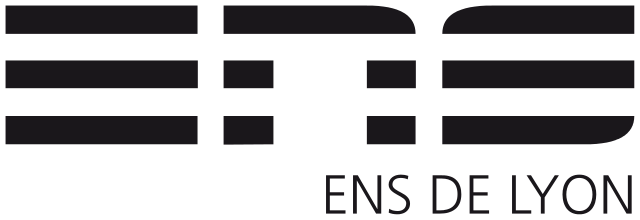
\includegraphics[height=2cm, keepaspectratio]{École_normale_supérieure_de_Lyon_Logo.svg.png}\\[1cm]

\textsc{\LARGE Research Internship report}\\[1.25cm]
\HRule \\[0.4cm]
{ \huge \bfseries The Hypercubic Manifold}\\[0.3cm]
{ \huge \bfseries in}\\[0.5cm] 
{ \huge \bfseries Homotopy Type Theory}\\[0.3cm]
\HRule \\[2cm]
\begin{minipage}{0.4\textwidth}
\begin{flushleft}
\emph{\Large \emph{\textbf{Author :}}}\\[0.2cm]
\textsc{\Large Dylan LAIRD}\\
\textit{Student at ENS Lyon}
\end{flushleft}
\end{minipage}
~
\begin{minipage}{0.4\textwidth}
\begin{flushleft}
\emph{\Large \emph{\textbf{Supervisers :}}}\\[0.2cm]
\textsc{\Large Samuel MIMRAM}\\
\textit{Full Professor at LIX, École Polytechnique}\\[0.1cm]
\textsc{\Large Émile OLÉON}\\
\textit{PhD student at LIX, École Polytechnique}\\
\end{flushleft}
\end{minipage}\\[0.5cm]

\begin{figure}[h]
    \begin{minipage}[c]{.46\linewidth}
        \centering
        
\includegraphics[height= 5cm]{École_polytechnique_signature.svg.png}
    \end{minipage}
    \begin{minipage}[c]{.46\linewidth}
        \centering
        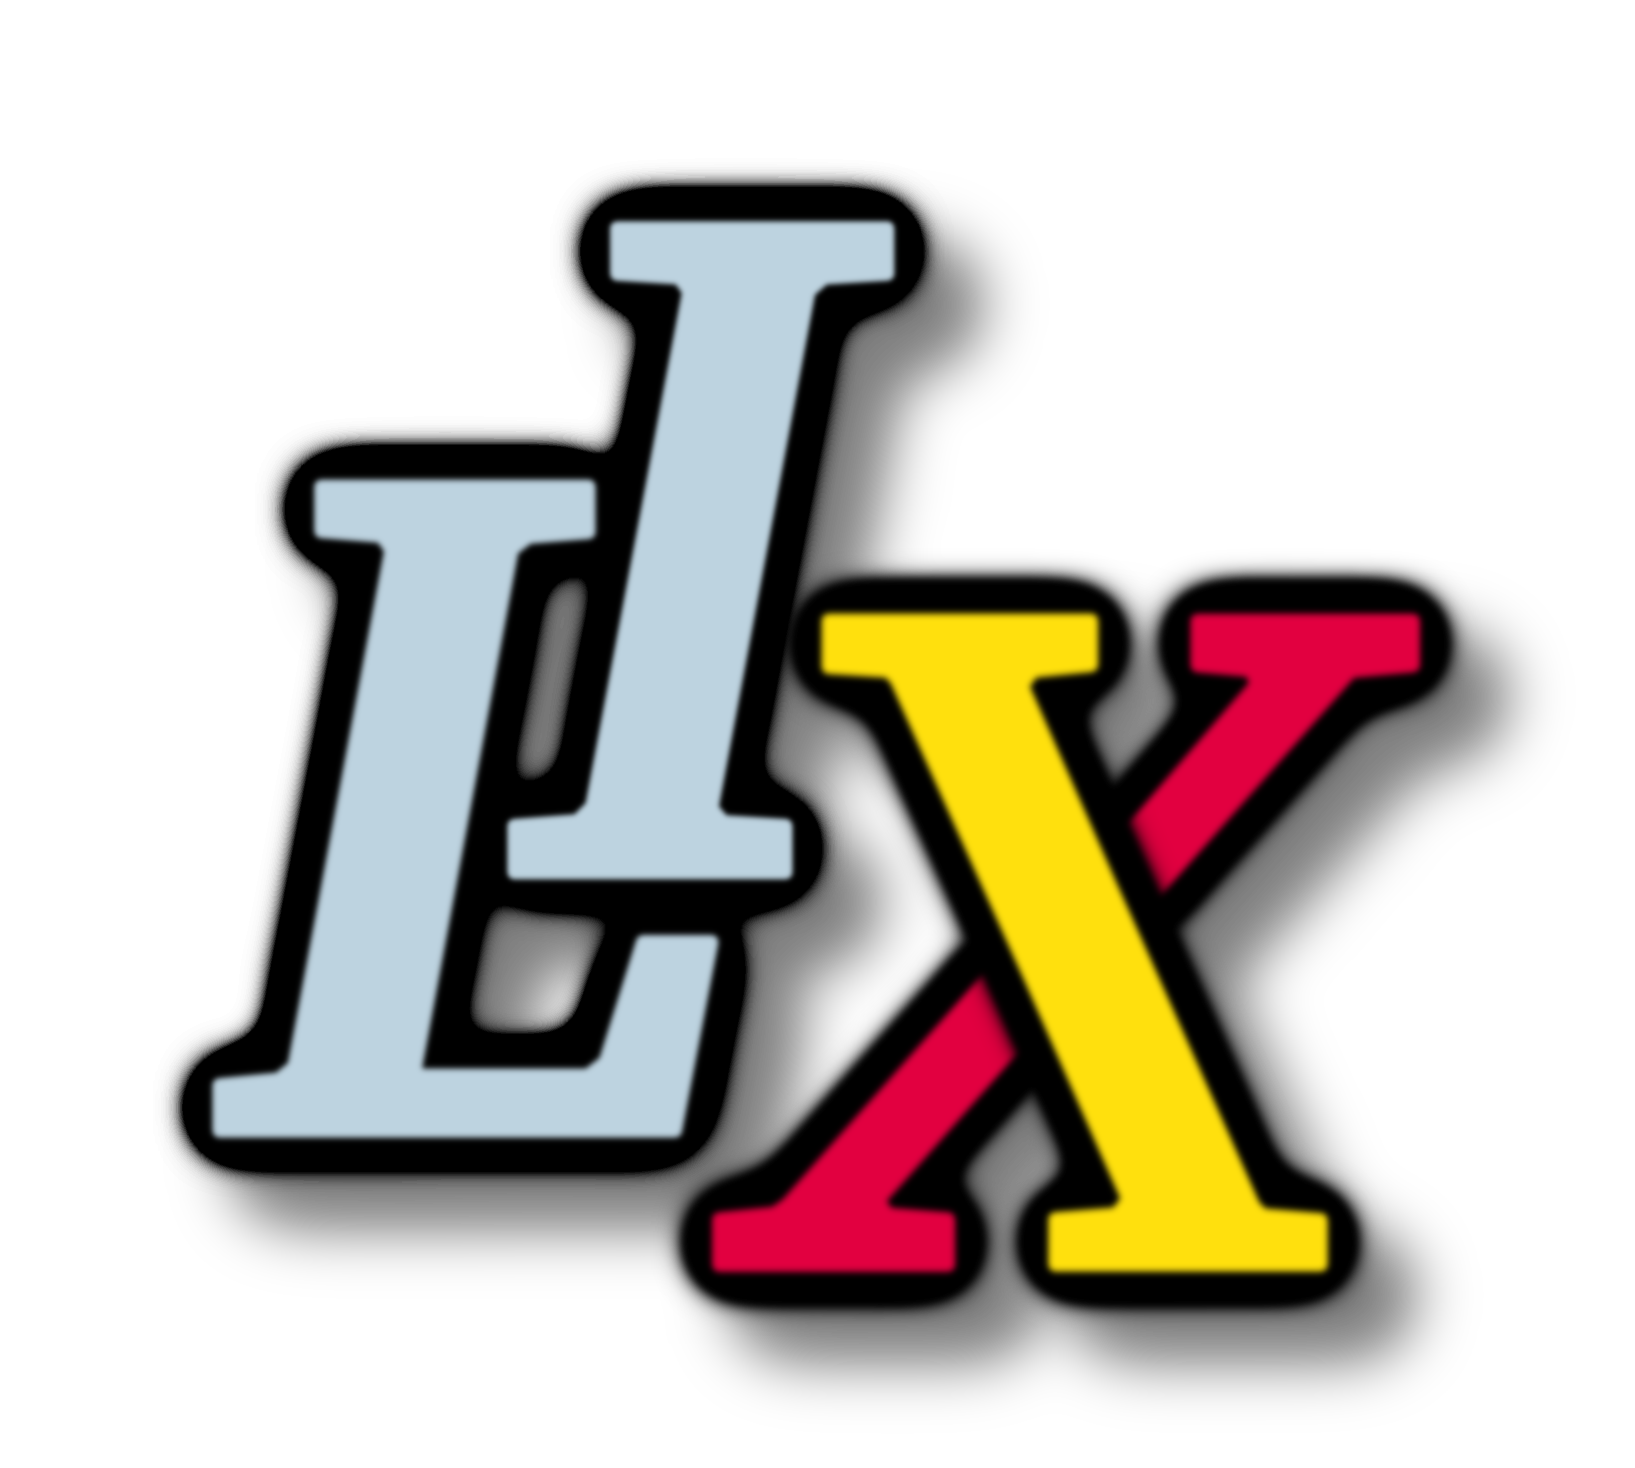
\includegraphics[height=5cm]{logo_lix.png}
    \end{minipage}
\end{figure}
\vfill % Fill the rest of the page with whitespace
\end{titlepage}
\tableofcontents
\section{Introduction}
\textbf{Homotopy Type Theory} (which I will often refer to as \textbf{HoTT} in this report) is a new field in mathematics and computer science, at the crossroad of \textbf{Type Theory}, \textbf{Homotopy Theory} and the \textbf{Foundations of Mathematics}. It is based upon a homotopical interpretation of \textbf{Martin-Löf's Type Theory}, with the addition of the \textbf{Univalence Axiom} and \textbf{Higher Inductive Types}, that allow one to proceed with univalent mathematics and doing homotopy theory within the synthetic framework of type theory.\\
The univalence axiom roughly states that equal types are precisely equivalent types (this will be made clearer later on). However, as it is often the case with type theory, we are interested in the computability of our system, and it appears that the univalence axiom does note compute. This is one of the motivation for the introduction of \textbf{Cubical type theory}, that gives a constructive interpretation of the univalence axiom.\\
The goal of this internship was to give a definition of the \textbf{hypercubic manifold} in HoTT/cubical type theory using the agda proof assistant and the cubical agda library \cite{cubicalagda} and to prove some further results about it. The hypercubic manifold \cite{hypercubic} is obtained as an adjunction space of a 3-dimensional hypercube. As shown in \cite{hypercubic}, it is obtained by gluing opposite faces of a cube with a quarter turn each time.\\
Homotopy type theory being a very atypical theory, it comes with a lot of new definitions, ideas and concepts. This makes it hard to summarize both the basic theory needed for the internship (roughly speaking, chapters 1,2,3,4,6,8 of the \textbf{HoTT Book} \cite{hott}) as well as the content of the internship itself in 20 pages. For that reason, this report will feature an important work of summarization of both basic and more advanced topics in HoTT (however many details and important results will be overlooked due to the little space), and the work I did myself during the internship might not take up the most important chunk of space in this report. All the formalized results, and attempts, obtained during the internship can be found on this github repository. This report wil be divided into 2 sections, the first one introducing the required HoTT concepts, and the second one tackling what was made during the internship.
\chapter{Pre-requesites}
The following part is aimed at giving a sufficent background for one to be able to understand the material from the internship. The presentation is very much inspired from the \textbf{HoTT Book} \cite{hott}. 
\begin{comment}
\section{Category Theory}
\subsection{Definitions and motivations}
\paragraph{Categories} A category $\mathcal{C}$ consists of a class of \textbf{objects}, a class of \textbf{arrows} or \textbf{morphisms} that each have a \textbf{source} and a \textbf{target} which themselves are objects of $\mathcal C$. For each object $A$ of $\mathcal{C}$, there is an \textbf{identity morphism} $1_A$, and those arrows should behave as we expect: if two arrows $f$ and $g$ satisfy $\mathrm{codom} f =\mathrm{dom} g$ then there is an arrow $g \circ f$ which is the composite, and composition of arrows is associative and identity morphisms behave as identity elements for this law.
\paragraph{Working examples}We will mainly be looking at two categories for now. The category $\textbf{Set}$ whose objects are sets and morphisms are function between these sets (we won't bother with the foundational aspects of why it is actually a thing that this category exists). As we will be dealing with homotopy theory, we should also be looking at the category $\textbf{Top}$ of topological spaces, and whose arrows are continuous maps between theses spaces (luckily, indentity maps are indeed continuous !).
\paragraph{Products}
In the category $\textbf{Set}$ one can take two sets $A$ and $B$ and look at the set $A\times B$. Category theory is the framework that allows to speak about these kind of constructions in a more general way. For instance, given a category $\mathcal{C}$ and two objects $A,B$ (those will be our standard notations from now on), we say that an object $X$ equipped with \textbf{projection morphisms} $\pi_1$ and $\pi_2i$ is a product of $A$ and $B$ if it satisfies the following \textbf{universal property}: for any object $Y$ and arrows $f : Y \rightarrow A$, $g : Y \rightarrow B$, there is a \textbf{unique} arrow $f \otimes g$ that makes the following diagram commute: 
\begin{center}
\[\begin{tikzcd}
	&&&& Y \\
	\\
	\\
	\\
	A &&&& X &&&& B
	\arrow["{\exists! f \otimes g}"{description}, dotted, from=1-5, to=5-5]
	\arrow["{\pi_2}", from=5-5, to=5-9]
	\arrow["{\pi_1}"', from=5-5, to=5-1]
	\arrow["g", from=1-5, to=5-9]
	\arrow["f"', shift right=2, from=1-5, to=5-1]
\end{tikzcd}\]
\end{center}
It is essential to note that the very fact that we demanded a \textbf{universal property} insures that the product of $A$ and $B$ is \textbf{unique up to isomorphism} (we will not prove it but it is an elementary exercise). We say that $X$ is \textit{universal} for the previous property. In the case of the category $\textbf{Set}$, one recovers the product set of $A$ and $B$ and the same goes for the category $\textbf{Top}$.\\
This is a general pattern that we will encounter throughout this section : we will define operations on objects of a certain category with universal properties that will ensure that they are unique up to isomorphism (which is all that matters). We will be looking at a few more categorical constructions that will be useful afterwards, and show what they allow us to do in homotopy theory.
\subsection{Push-out diagrams}
Given a span :
\begin{center}
    \[\begin{tikzcd}
	Z &&& Y \\
	\\
	\\
	X
	\arrow["g", from=1-1, to=1-4]
	\arrow["f"', from=1-1, to=4-1]
\end{tikzcd}\]
\end{center}
the pushout of morphisms $f,g$ consists of an object $P$ with morphisms $i_1,i_2$ such that the following diagram commutes and that $(P,i_1,i_2)$ is universal with respect to this diagram : 
\begin{center}
    \[\begin{tikzcd}
	Z &&& Y \\
	\\
	\\
	X &&& P
	\arrow["g", from=1-1, to=1-4]
	\arrow["f"', from=1-1, to=4-1]
	\arrow["{i_1}"', from=4-1, to=4-4]
	\arrow["{i_2}", from=1-4, to=4-4]
\end{tikzcd}\]
\end{center}
In the category $\textbf{Set}$, with $Z$ being the $\emptyset$, one recovers the \textbf{disjoint union} of sets. In a general case, one should think of $P$ as being a sum of $X$ and $Y$ where elements of $Z$ corresponding through $f$ and $g$ are identified. In the category $\textbf{Top}$, pushout exists and $P$ consists of $X \bigoplus Y / \equiv$ where $\equiv$ is the equivalence relation generated by $\{i_1(f(z)) = i_2(g(z)) \mid z \in Z \}$.
\paragraph{The 1-skeleton of the hypercubic manifold} Later on, we will try and define the hypercubic manifold as a \textbf{pushout space}. For now, let's look at how one can obtain the \textbf{1-skeleton} of this manifold using a simple pushout. We aim to build a space with the following elements: 
\begin{center}
    \begin{itemize}
        \item two points $\textbf{blue}$ and $\textbf{white}$
        \item four edges $\textbf{red}^E$, $\textbf{blue}^E$, $\textbf{yellow}^E$, $\textbf{green}^E$ from point $\textbf{white}$ to  $\textbf{blue}$
    \end{itemize}
\end{center}
To do so let $\mathrm{Edges} = \{\textbf{red}^E,\textbf{blue}^E,\textbf{yellow}^E,\textbf{green}^E\}$, $\mathrm{Source}=\{\textbf{white}\}$ and $\mathrm{Target}=\{\textbf{blue}\}$. The the following pushout 
\end{comment}
\section{Type Theory}
In type theory, all that we manipulate are \textbf{types} $A,B$ and \textbf{terms} of those types for instance $a : A$ and we have \textbf{type forming rules} to form terms of types from already existing types. The most infamous example is the one of the natural integers defined inductively by:
\begin{itemize}
    \item $0 : \mathbb N$
    \item $\mathrm{suc}: \mathbb N \rightarrow \mathbb N$
\end{itemize}
The type of natural integers also comes with its well-known \textbf{induction principle}. In type theory, since all we work with are types, we will also have induction principles that come along any type we define.\\
It is to be noted that \textbf{equality} plays a central role in Type Theory. We distinguish two kind of equalities, \textbf{definitional equality}, which we will note $\equiv$, it isn't an actual part of Type Theory but lives at the same level as judgements "$a : A $". For example, setting $f$ to be the function $x \mapsto x^2 $ (say over the integers), for any integer $a$ we would then have $f a \equiv a^2$, which is to be read as "$f a$ is definitionnaly equal to $a^2$".\\
It must not be mistaken with \textbf{(propositional) equality} which we will take a closer look at later on. For now, let's just recall that in Type Theory every object is a type and so, for two elements $a,b :A$ we can build the type $a =_A b$, namely the \textbf{identity type} of $a$ and $b$, and to prove that $a$ and $b$ are equal elements (of $A$), one has to produce an element $p : a=_A b$.
\subsection{Function types}
Given two types $A,B$, one can build the \textbf{type} $A \rightarrow B$ of functions from $A$ to $B$. To build an element of that type, one needs to give an expression $\Phi(x)$ such that : $a : A \vdash \Phi(a) : A$, and can define an element $f$ with the following syntax: 
$$f(x) :\equiv \Phi(x) \hspace{5pt}\text{(such definitions yield \textbf{definitional} equalities)}$$
\subsection{Universes, type families and dependent function types}
To introduce types more formally, we need to talk about \textbf{universes}, which, as in set theory, allow us to avoid unsoundness problems (such as Russel paradox). Details need not concern us here, let's just get straight to the point: we suppose that we have a \textbf{cumulative hierarchy} of universes $\mathcal{U}_i$, and elements of such a universe are themselves some type. Hence, giving ourselves a type $A$ is tantamount to giving ourselves an element from some universe $\mathcal{U}$ (we will not mention the level from now on).\\
 Universes allow us to introduce \textbf{Type familes}, that is, a type family over a type $A$ is a function of type $A \to \mathcal{U}$.
 \paragraph{Dependent function types ($\Pi$-types)}
 For now, let's note that we can talk about \textbf{dependent functions}. Given a type $A$ and a type family $C: A \rightarrow \mathcal{U}$, one can build the type of dependent functions over $A$, whose codomain can vary along $C$: 
$$\prod_{x : A} C(x)$$
The formation rule is the same as before, one can build an element $f$ of type $\prod_{x : A} C(x)$ with an expression $\Phi(x)$ such that $a : A \vdash \Phi(a) : C(a)$ and by setting $f(x) :\equiv \Phi(x)$.
\subsection{Product types}
Given types $A,B : \mathcal{U}$ one can build their \textbf{cartesian product type} $A \times B : \mathcal{U}$. The formation rule is as natural as it gets, given $a : A$ and $b : B$ one can form $(a,b) : A \times B$. We shall now encounter our first \textbf{recursion principle}, which in the general case, encompasses how to build \textbf{non-dependent functions} out of a certain type. The recursion principle for product types allows us to define a function over $A\times B$ by specifiying its values on pairs $(a,b)$. This principle can be phrased in a proper type theoretic way as follows:
$$\mathrm{rec}_{A\times B} : \prod_{C : \mathcal{U}} (A \rightarrow B \rightarrow C) \rightarrow A\times B \rightarrow C$$
with the defining equation:
$$\mathrm{rec}_{A\times B}(C,f,(a,b)) :\equiv f(a)(b)$$ 
From now on, we will only refer informally to the recursion and induction principles without writing them out formally.\\
As an example, we can now define the first projection $\mathrm{pr}_1 : A\times B \rightarrow A$ by $\mathrm{pr}_1(a,b) :\equiv a$ and the second projection by $\mathrm{pr}_2 (a,b) :\equiv b$.\\ 
It is time to elaborate on a central philosophical aspect of Type Theory. In classical mathematics, one constructs the product of sets $A$ and $B$ with the sets of all pairs of the form $(a,b)$. In Type Theory however, we have not (yet) seen any mention that the type $A\times B$ is the "type of all pairs $(a,b)$", meaning that there may be some element $x : A \times B$ which is \textit{not} a pair $(a,b)$. In fact, it turns out that we do have a \textbf{uniqueness principle} for product types, which ressembles to what we would expect, however, as we are working within Type Theory we cannot expect it to be more than a \textbf{propositional uniqueness principle}. Before stating it, we need to take a look at the \textbf{induction principle} for product types, which in the general case encompasses how to build \textbf{dependent functions} out of a certain type. In our case, as for the recursion principle, defining a dependent function $f$ over $A \times B$ only requires to define over pairs $(a,b)$.\\
We are now set to prove the \textbf{propositional uniqueness principle of product types} :
\begin{prop}
  For any $x : A \times B$, one has : $x =_{A \times B} (\mathrm{pr}_1(x),\mathrm{pr}_2(x))$, that is, we have a dependent function:
  $$\mathrm{uniq}_{A\times B} : \prod_{x : A \times B} \big(x =_{A \times B} (\mathrm{pr}_1(x),\mathrm{pr}_2(x))\big)$$
\end{prop}
\begin{proof}
     Here, we want to build the dependent function $\mathrm{uniq}_{A\times B}$. We will hence be using the induction principle for product types, which states that we need to exhibit for any pair $a : A$ and $b : B$ an element$f(a)(b)$ of type $(a,b)=_{A \times B} (\mathrm{pr}_1((a,b)),\mathrm{pr}_2(a,b))$. However,  $(\mathrm{pr}_1((a,b)),\mathrm{pr}_2(a,b))$ is \textbf{definitionnally} equal to $(a,b)$ (by the definition that we have given of the projections) and so we are reduced to exhibit $f(a)(b) : (a,b)=_{A \times B} (a,b)$.\\ 
     We shall now use a fact that we haven't seen yet about identity types, but that should seem familiar, is that for any $x$ of some type $X$ the type $x=_{X}x$ is inhabited by an element $\mathrm{refl}_x$. We can therefore set $f(a)(b) :\equiv \mathrm{refl}_{(a,b)}$ to terminate the proof.
\end{proof}
\subsection{Dependent pair types ($\Sigma$-types)}
Given a type $A$ and a type family $B : A \rightarrow \mathcal{U}$, one can construct the \textbf{dependent pair type}: 
$$\sum_{x : A} B(x)$$
To form an element of such a type, one needs elements $a : A$ and $b : B(a)$, resulting in an element $(a,b) : \sum_{x : A} B(x)$. It should be noted that theses types are a generalization of product types and that for the constant type family at $B$, $C :\equiv \lambda (x : A).B$ we have $\sum_{x = A} C(x)\equiv A \times B$.\\
As for product types, one can define dependent and non dependent functions $f$ over the type $\sum_{x : A} B(x)$ by specifiying its values on dependant pairs $(a,b)$ where $b:B(a)$.\\ 
The recursion principle allows us to define (again) the first projection $\mathrm{pr}_1 : \sum_{x : A} B(x) \rightarrow A$ by $\mathrm{pr}_1 (a,b) :\equiv a$.\\
However, defining the second projection is now a bit trickier since it should have the type $\prod_{p : \sum_{x : A} B(x)} \mathrm{pr}_1(p)$, making it a dependent function. It thus requires the use of the induction principle, and we can define it by its values on dependant pairs by $\mathrm{pr}_2(a,b) :\equiv b$.
\subsection{Coproduct types}
Given types $A$ and $B$, one can define their coproduct type $A+b$ inductively with two constructors:
\begin{itemize}
  \item inl : $A \rightarrow A+B$
  \item inr : $B \rightarrow A+B$
\end{itemize}
It should be thought of as containing two disjoints copies of $A$ and $B$. The induction principle is here tantamount to \textbf{case analysis}, to define a function over $A+B$ one needs to specify its value on elements $inl(a)$ for $a:A$ and on elements $inr(b)$ for $b:B$. 
\subsection{Propositions as types}
We will be looking at Type Theory in details in the next section, for now let's just take a look at the following table showing the \textbf{Proposition as Types correspondance} also known as the \textbf{Curry-Howard isomorphism}:
\begin{center}
\begin{tabular}{|c|c|}
\hline Types & Logic  \\
\hline$A$ & $A$ is a proposition  \\
\hline$a: A$ & $a$ is a proof of $A$ \\
\hline $\textbf{0},\textbf{1}$ & $\perp, \top$ \\
\hline$A+B$ & $A \vee B$  \\
\hline$A \times B$ & $A \wedge B$  \\
\hline$A \rightarrow B$ & $A \Rightarrow B$ \\
\hline$A \rightarrow \textbf{0}$ & $\lnot A$ \\
\hline
\end{tabular}
\end{center}
This correspondence shows the similarity in between type forming rules and rules of propositional logic when seeing "propositions as types" and vice versa. For instance, if one wants to build a term of type $A \times B$, one needs a term $a : A$ and a term $b : B$ to form $(a,b) : A \times B$. Similarly, to prove the proposition $A \land B$, one needs a proof of $A$ and a proof of $B$. \\
In the same way, building a function $f : A \rightarrow B$ (or a proof of $A \implies B)$ requires to be able to build an element of $B$ (a proof of $B$) given an element an $A$ (given a proof of $A$).\\
Under this correspondence, it also makes sense to talk about a predicate over a type $A$ for a type family $P : A \rightarrow \mathcal{U}$. Then, for $a :A$ the type $P(a)$ corresponds to the propositions "$P$ holds for $a$". We then have the following correspondance : 
\begin{center}
  \begin{tabular}{|c|c|}
  \hline Types & Logic  \\
  \hline$\prod_{x : A} P(x)$ & For all $x :A$, $P(x)$ holds  \\
  \hline$\sum_{x : A} P(x)$ & There exists $x : A$ such that $P(x)$ holds\\
  \hline
  \end{tabular}
\end{center} 
One can also think of the type $\sum_{x: a} P(x)$ as the type of all $x : A$ such that $P(x)$ holds.
\paragraph{Semi-groups}
Let's illustrate how our type formers and the proposition as types interpretation allows us to define some mathematical structure. We call a \textbf{semigroup} a type $A$ equipped with an associative binary operation $m : A \times A \rightarrow A$. Under the proposition as types interpretation, the proposition that $m$ is associative is described by the following type : 
$$\mathrm{isAssoc}(m) : \prod_{x,y,z : A }m(x,m(y,z))=m(m(x,y),z)$$
Then, a semigroup structure is given by a type $A$, a binary operation $m$ over $A$ and a proof that $m$ is associative, and so we can the define the type of semigroups over a universe $\mathcal{U}$ by : 
$$\mathrm{SemiGroup} :\equiv \sum_{A : \mathcal{U}} \sum_{m : A \times A \rightarrow A} \mathrm{isAssoc}(m)$$
\subsection{Identity types family}
For a type $A: \mathcal{U}$ we have a type family $\mathrm{Id} : A \rightarrow A \rightarrow \mathcal{U}$ (we will write $x=y$ for $\mathrm{Id}_A(x)(y)$ if the context is clear) and a dependent function called reflexivity:
$$\mathrm{refl} : \prod_{x : A} (x=x)$$
For two elements $x,y : A$ we say that $x=y$ if the type $x=_A y$ is inhabited.
\paragraph{Path induction}
Let's illustrate the induction principle for \textbf{indentity type families}, called path induction by proving that functions preserve equals.
\begin{prop}
Let $f : A \rightarrow B$, then for any $x,y :A$ there is a function :
$$\mathrm{ap}_f : (x=y) \rightarrow (f(x)=f(y))$$ 
\end{prop}
\begin{proof}
The \textbf{path induction} principle indicates that to prove this predicate for any $x,y : A$ and $p : x=y$, we only need to prove it when $x\equiv y$ and $p \equiv \mathrm{refl}_x$. We thus want an element of type  $f(x) = f(y)$, but under our assumptions $f(x) \equiv f(y)$ and so $(f(x)=f(y)) \equiv (f(x)=f(x))$ and so by setting $\mathrm{ap}_f(\mathrm{refl}_{f(x)}) :\equiv \mathrm{refl}_{f(x)}$ we can terminate the proof. 
\end{proof}
Under the proposition as types interpretation, this induction principle states that to prove a predicate over a \textit{family} of identity types, namely $P : \prod_{x,y : A} (x=y) \rightarrow \mathcal{U}$, it suffices to prove it in the case where both ends are definitionnaly equal and that their proof of equality is reflexivity. There is another (but equivalent) induction principle called \textbf{based path induction} where one of the ends $x$ or $y$ is fixed to a certain element of $A$. However, in both these versions it is crucial to note that the induction principle is about a \textit{family} of identity types, and not one identity type with both ends fixed.\\
As an example, this principle does \textit{not} imply that every identity type is "trivial". Such a statement would go along those lines "for $a : A$ and $p: a=a$ we have that $p = \mathrm{refl}_a$". This statement isn't about identity types \textit{families} so our induction principle does not apply.
\section{Homotopy Type Theory}
\subsection{Classical homotopy theory}
In classical topology, if $X$ is a topological space and $x,y$ are points of $X$, a \textit{path} between $x$ and $y$ is a continuous map $p : [0,1] \rightarrow X$ such that $p(0)=x$ and $p(1)=y$.\\
A \textbf{homotopy} in between two paths $p,q$ from $x$ to $y$ is then a continuous map $H : [0,1] \times [0,1] \rightarrow X$ such that $(x \mapsto H(0,x) )= p$, $(x \mapsto H(1,x)) = q$ and that for any $t \in [0,1]$, $x\mapsto H(t,x)$ is a path from $x$ to $y$. A homotopy between paths $p$ and $q$ should be thought of as a continuous deformation between those two paths. Moreover, there are two natural operations on paths:
\begin{itemize}
    \item \textbf{concatenation} : if $p$ is a path from $x$ to $y$ and $q$ is a path from $y$ to $z$ then there is a path $p \cdot q$ from $x$ to $z$ defined by following $p$ then $q$
    \item \textbf{inversion} : if $p$ is a path from $x$ to $y$ then we can follow the path $p$ the other way round to obtain its inverse $p^{-1}$ which is a path from $y$ to $x$
\end{itemize}
The special case of \textbf{loops} is obtained by looking at path with the same starting point and ending point. Then the two previous operations are always defined on loops with the same basepoint $x$. More interestingly, those operations are consistant with homotopy of loops and the constant path at point $x$ acts as a unit element.
We therefore obtain a group structure for loops (up to homotopy) at basepoint $x$ which is called the \textbf{fundamental group} of $X$ at point $x$ and denoted by $\pi_1(X,x)$.\\
Since homotopies themselves are continuous maps of topological spaces, one can look at homotopies between homotopies and so on, and we can define some \textbf{higher homotopy groups} $\pi_2,\pi_3,\ldots$. Those groups are interesting since they are algebraic invariant of homeomorphical, or more precisely, homotoically equivalent spaces.
\paragraph{Homotopy type theory} So, how does it relate to our type theory? At first, one could think of our types as set, like the example of $\mathbb N$ would suggest, and for instance the product type would be analogous to the product set. However, in the previous section we have seen identity types and how these types are generally speaking \textit{not} trivial (that is, every inhabitant is $\mathrm{refl}$).  Thanks to identity types, we would rather think of types as spaces as it is suggested by the following table:
\begin{center}
\begin{tabular}{|c|c|}
\hline Types & Topology  \\
\hline$A$ & a space $A$   \\
\hline$a: A$ & $a$ is a point of $A$ \\
\hline $p : x=_A y$ & $p$ is a path from $x$ to $y$ in the space $A$ \\
\hline
\end{tabular}
\end{center}
The particular case where types behave like sets, as it is for the type of natural integers, is here recovered through the particular case of \textit{discrete spaces}. However, this does not make sense until we have proven some additional properties about identity types that should relate to the ones of paths in topology.
\begin{figure}[h]
  \centering
  \begin{tikzpicture}
    \draw (0,0) ellipse (3.5cm and 2cm);
    \filldraw (-2.5,0) circle (1.5pt) node [below left] {$x$};
    \filldraw (2.5,0) circle (1.5pt) node [below right] {$y$};
    \filldraw [pattern={Lines[angle=60, distance=8pt]}] (-2.5,0) .. controls (-1,1.5) and (1,1.5) .. (2.5,0) .. controls (1,-1.5) and (-1,-1.5) .. (-2.5,0) -- cycle;
    \draw [thick, double] (0,1.152) -- (0,-1.152) node [at start, above] {$p$} node [midway, right] {$r$} node [at end, below] {$q$};
    \node (A) at (3.3,1.5) {$A$};
  \end{tikzpicture}
  \caption{a type $A$ with points $x,y : A$, two paths $p,q: x=_A y$ and a homotopy $r : p =_{x=_A y} q$}
\end{figure}
\subsection{Paths}
In short, we have the following correspondence in between equality types in Type Theory and paths in omotopy theory:
\begin{center}
\begin{tabular}{|c|c|}
  \hline Equality & Homotopy \\
  \hline reflexivity & constant path \\
  \hline symmetry  & path inversion \\
  \hline transitivity & concatenation of paths \\
  \hline
\end{tabular}
\end{center}
Let's get into a bit more details about operations on equality types, one can prove every statement within this section by easy path inductions.
\paragraph{Symmetry} Given a path $p : x =_A y$, one has an inverse path $p^{-1} : y =_A x$ such that for any $x$, $\mathrm{refl}_x^{-1} \equiv \mathrm{refl}_x$.
\paragraph{Transitivity} Given paths $p : x =_A y$ and $q : y =_A z$ one has a concatenated path $p \cdot q : x =_A z$ such that for any $x$, $\mathrm{refl}_x \cdot \mathrm{refl}_x \equiv \mathrm{refl}_x$.

What's crucial about the paths operations we defines is that, as it should be expected, they are well behaved up to homotopy, allthough in a type theoretic way. This is encapsulated within the following properties, that can once again be proven by path inductions (the fact that these properties hold relies on how the operations have previously been defined, more details can be found in the HoTT Book\cite{hott}).
\begin{prop}
  Given a type $A$, $x,y,z,w : A$ and $p : x=y$, $q : y=z$, $r : z=w$, we have the following:
  \begin{itemize}
    \item $p = p \cdot \mathrm{refl}_y$ and $ \mathrm{refl}_x \cdot p = p$. 
    \item $p^{-1} \cdot p = \mathrm{refl}_y$ and $p \cdot p^{-1} = \mathrm{refl}_x$.
    \item $(p^{-1})^{-1} = p$
    \item $(p \cdot q) \cdot r = p \cdot (q \cdot r)$ (that is associativity of concatenation)
  \end{itemize}
\end{prop}
To end this section, let's note that we have already proven that functions preserve equal elements, in view of the homotopical interpretation of type theory this means that functions preserve paths, which should be thought of as \textbf{continuity for every non-dependent functions}. Additionally, we should note that \emph{non-dependent} functions behave \textit{functorially} on paths, yielding some natural equalities (such as $f(\mathrm{refl}_x)=\mathrm{refl}_{f(x)}$) that we won't be going through here.
\subsection{Transport and fibrations}
Thanks to the homotopical interpretation, we can now set out to do homotopy theory within type theory.\\
In classical logic, one of the main properties of equality is the \textbf{Leibniz law}, that is if $a=b$ and we have $P(a)$ then $P(b)$ holds. This is also true in HoTT, but can be understood in a different way in wake of the homotopy interpretation. Recalling that a predicate over a type $A$ in type theory is given by a type family $P : A \rightarrow \mathcal{U}$, one can define the following function by path induction :
$$\mathrm{transport}^P : \prod_{a,b : A} \prod_{p : a=_A b} P(a) \rightarrow P(b)$$
Under the proposition as types interpretation, this is precisely the Leibniz Law. We may write $\mathrm{transport}^P(a,b,p)$ as $p_*$ if the context is clear.\\
Now, in classical homotopy theory a \textbf{fibration} is defined as a continuous map $p : E \rightarrow B$ of topological spaces satisfying a certain path lifting property from the base space $B$ to the total space $E$. For $b : B$, $p^{-1}(B)$ is called the \textbf{fiber} at or over the point $b$. In HoTT, one can recover fibrations via type families. More precisely, given a type family $P : A \rightarrow \mathcal{U}$, the space $ \sum_{x : A} P(x)$ equipped with the first projection $\mathrm{pr}_1 : \sum_{x : A} P(x) \rightarrow A$ is a fibration with base space $A$ in the following sense : 
\begin{prop}[Path lifting]
  Given $x : A$ and $u : P(x)$, for any $y : A$ and $p : x=y$, one has a path 
  $$\mathrm{lift}(p,u) : (x,u) = (y,p_*(u))$$
  such that $\mathrm{pr}_1(\mathrm{lift}(p,u)) = p$.
\end{prop}
\begin{center}
  \begin{tikzpicture}[scale=0.865]
    \draw (0,7) ellipse (4.4cm and 2.5cm);
    \draw (-1.7,7) ellipse (1.15cm and 1.05cm);
    \draw (1.7,7) ellipse (1.15cm and 1.05cm);
    \filldraw (-1.7,7) circle (1.5pt) node [above left] {$u$};
    \filldraw (1.7,7) circle (1.5pt) node [above right] {$p_*(u)$};
    \draw (-1.7,7) .. controls (-1,8) and (1,8) .. (1.7,7) node [midway, above] {$\mathrm{lift}(p,u)$};
  
    \draw [dash pattern=on 5pt off 3pt] (-1.7,0) -- (-1.7,7) (1.7,0) -- (1.7,7);
    \draw [very thick, ->] (-3,4.5) -- (-3,1.5) node [midway,left] {$\mathrm{pr}_1$};
  
    \draw (0,0) ellipse (4.4cm and 1.5cm);
    \filldraw (-1.7,0) circle (1.5pt) node [below left] {$x$};
    \filldraw (1.7,0) circle (1.5pt) node [below right] {$y$};
    \draw (-1.7,0) .. controls (-0.7,0.7) and (0.7,0.7) .. (1.7,0) node [midway, above] {$p$};
     
    \node (A) at (4.5,-1.5) {$A$};
    \node (B) at (5,5.5) {$\displaystyle\sum_{a:A} B(a)$};
    \node (C) at (-3.5,7) {$B(x)$};
    \node (D) at (3.5,7) {$B(y)$};
  \end{tikzpicture}
\end{center}
This shows that paths in the base space of $\sum_{x : A} P(x)$ can be lifted in the expected way. Indeed, the Leibniz law we previously stated shows how one can identify elements from fibers $P(x)$ and $P(y)$ with respect to a certain path $p : x=y$, and the path lifting property tells us exactly that given a path $p: x = y$ in the base space and a point $u : P(x)$ in the fiber over $x$, we have a path in the total space between $(x,u)$ and the point in the total space you should expect that it is transported to via $p$, namely $(y,p_*(u))$. The fact that $\mathrm{pr}_1(\mathrm{lift}(p,u)=p)$, tells us in a way that the path $\mathrm{lift}(p,u)$ in the total spaces \textit{lies over} the path $p$ in $A$ (this should prove to be useful later on).
\subsection{Equivalences and the univalence axiom}
Under the homotopical interpretation we have seen that equalities should be understood as paths. In topology, we have a notion of \textbf{homotopy} between functions, that one can naturally recover in HoTT:
\begin{mydef}[Homotopy]
  Given $P : A \rightarrow \mathcal{U}$ and $ f,g : \prod_{x : A} P(x)$ we define the type of homotopies between $f$ and $g$ by
  $$(f \sim g) :\equiv \prod_{x : A} (f(x)=g(x))$$
\end{mydef}
A priori, this is \textit{not} the same as the type $f =g$. Now, let's move on to types : what exactly is an equality between types ? Firs, as types can be seen as inhabitant of a certain universe type, we do have equality types in between types themselves.
In topology, thanks to homotopies, one can define homotopically equivalent spaces as spaces $X,Y$ with two maps $f : X \rightarrow Y$ and $g : Y \rightarrow X$ such as both their composites are homotopical to the identity maps. Allthough it would be natural, this is \textit{not} what is retained as the definition for equivalence of types, but corresponds to so called \textbf{quasi-equivalences} of types. We won't be defining equivalence of types here, but it goes along the lines of the one of quasi-equivalences. In fact, and that is what should be taken away, one can build an equivalence from a quasi-equivalence and vice-versa. We will often be building quasi-equivalences to show that two types are equivalent. We will write the type of equivalences in between $A$ and $B$ as $A \simeq B$.\\
\paragraph{Univalence}
If we talked about equivalences first, it is because they play a fundamental role in HoTT thanks to the univalence axiom. One should expect equal types to be equivalent and that is the case, meaning that we have a function: 
$$\mathrm{idToEquiv : A = B \rightarrow} A \simeq B$$
Now, the \textbf{univalence axiom} consists in giving ourselves an arrow in the other direction:
$$\mathrm{ua} : A \simeq B \rightarrow A = B$$
And moreover, $\mathrm{ua}$ is such that it is a quasi-inverse to $\mathrm{idToEquiv}$ meaning that they are at turn equivalences, hence : 
$$(A \simeq B) \simeq  (A = B)$$
This whole univalence axiom, proposed by \textit{Vladimir Voevodsky}, allows us to identify equivalent types, as it usually done, allthough in an informal way, in classical mathematics. 
\subsection{Characterizing equality types in type formers}
We have previously seen that in a product type $A \times B$, given a path $p : x=y$, we can apply $\mathrm{pr}_1$ and $\mathrm{pr}_2$ to obtains paths $\mathrm{pr}_1(p) : \mathrm{pr}_1(x)=_A \mathrm{pr}_1(y)$ and $\mathrm{pr}_2(p) : \mathrm{pr}_2(x)=_B \mathrm{pr}_2(y)$. This allows us to define a function of type : 
$$ (x =_{A\times B} y) \rightarrow (\mathrm{pr}_1(x)=_A \mathrm{pr}_1(y)) \times (\mathrm{pr}_2(x)=_B \mathrm{pr}_2(y))$$
In fact, it turns out that it is an equivalence:
\begin{theorem}
The function previously defined is an equivalence so one has :
$$(x=_{A \times B} y) \simeq (\mathrm{pr}_1(x)=_A \mathrm{pr}_1(y)) \times (\mathrm{pr}_2(x)=_B \mathrm{pr}_2(y))$$
\end{theorem}
The conclusion of this theorem is pretty natural, equalities in product types are exactly pairwise equalities, or, under the homotopical interpretation, paths in a product are exactly pairs of paths.\\
Things get a bit more trickier when looking at $\Sigma$-types. Given a type family $B : A \rightarrow \mathcal{U}$, what do equalities in $\sum_{x : A} B(x)$ look like ? To answer this specific question , we need to elaborate a bit more on the notion of paths lying over other paths.
\paragraph{Paths over paths} Given a type family $P : A \rightarrow \mathcal{U}$ and a path $p : x=_A y$ we have a fibration which total space is $\sum_{x : A} P(x)$. Given a dependent function $f : \prod_{x :A } P(x)$, we would like to apply $f$ to $p$ in order to obtain a path $f(p) : (x,f(x))=f(y,f(y))$ in the total space of our fibration, lying over $p$. The previous proposition already gives a canonical path lying over $p$, namely $\mathrm{lift}(p,(f(x)) : (x,f(x)) = (y,p_*(f(x)))$, so, essentially, any path lying over $p$ between $((x,f(x)))$ and $(y,f(y))$ should factor through this canonical path $\mathrm{lift}(p,f(x))$. Up to equivalence, this would mean providing a path between points $p_*(f(x))$ and $f(y)$ lying in the fiber $P(y)$. And, as it should be expected, dependent functions yield such paths : 
\begin{prop}
Given $f : \prod_{x : A} P(x)$ and $x,y : A$, one has a map : 
$$\mathrm{apd}_f : \prod_{p : x=_A y} p_*(f(x))=f(y)$$
\end{prop}
Now, given a path $p :w =_{\sum_{x : A} B(x)} w'$, we can apply the (non-depedent) function $\mathrm{pr}_1$ to obtain a path $\mathrm{pr}_1(p) : \mathrm{pr}_1(w) =_A \mathrm{pr}_1(w')$, and thanks to the previous proposition and using the dependent function $\mathrm{pr}_2$, we obtain a path between $\mathrm{pr}_1(p)_*(\mathrm{pr}_2(w))$ and $\mathrm{pr}_2(w')$ lying in the fiber $B(\mathrm{pr}_1(w'))$. This, as previously seen is a path between $\mathrm{pr}_2(w)$ and $\mathrm{pr}_2(w')$ lying over the path $\mathrm{pr}_1(p)$. This allows us to define a map of type : 
$$w=_{\sum_{x : A} B(x)} w' \rightarrow \sum_{p : (\mathrm{pr}_1(w)=_A \mathrm{pr}_1(w'))} (p_*(\mathrm{pr}_2(w))=\mathrm{pr}_2(w'))$$
Once again, it turns out that this map is an equivalence,
\begin{theorem}
Let $B : A \rightarrow \mathcal{U}$ be a type family over $A$ and $w,w'$ be points of $\sum_{x : A} B(x)$, then there is an equivalence :
$$(w=_{\sum_{x : A} B(x)} w') \simeq \sum_{p : (\mathrm{pr}_1(w)=_A \mathrm{pr}_1(w'))} (p_*(\mathrm{pr}_2(w))=\mathrm{pr}_2(w'))$$
\end{theorem}
This means that an equality between two points $w$ and $w'$ is given by a path $p$ in $A$ between their first components and a path from $\mathrm{pr}_2(w)$ and $\mathrm{pr}_2(w')$ in the total space lying over this specific path $p$.
\subsection{Higher Inductive Types}
We have already seen an example of an inductive type : $\mathbb N$. When describing \textbf{higher inductive types}, we allow ourselves to use constructors that are not only points of the type, but also paths, paths between paths and every kind of higher paths one could think of. Those are especially useful when describing some concrete topological spaces, or constructions from topological spaces. Recall that in mathematics, one can define the circle $\mathbb{S}^1$ as the interval $[0,1]$ where points $0$ and $1$ indentified. This in fact gives two examples of HITs. The first one, is the interval type $I$ given by the following description:
\begin{itemize}
  \item $0 : I$
  \item $1 : I$
  \item $\mathrm{glue} : 0=_I 1$
\end{itemize}
And the second one is the circle type $\mathbb{S}^1$ : 
\begin{itemize}
  \item $\mathrm{base} : \mathbb{S}^1$
  \item $\mathrm{loop} : \mathrm{base} =_{\mathbb{S}^1} \mathrm{base}$
\end{itemize}
\begin{figure}[h]
  \begin{center}
    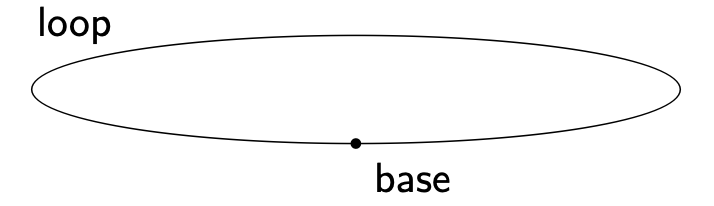
\includegraphics[height=2cm]{images/circle.png}
    \caption{The circle as a HIT (source: \cite{hott} chapter 6)}
  \end{center}
\end{figure}
Then, one could ask what induction principles would look like for HITs? We are able to describe induction principles on any given HIT, however, as there isn't really any generic description of what a HIT is, there is no general framework to answer this question. So, let's take a look at the case of the circle $\mathbb{S}^1$. The recursion principle for the circle states that to define a (non-dependent) map out of the circle to a type $A$ equipped with a point $a :A$ and a path $ p : a=_A a$ then there is a unique map $f : \mathbb{S}^1$ such that $f(\mathrm{base}) \equiv a$ and $\mathrm{ap}_f(\mathrm{loop}) =p$ (there is actually a case as to whether those equalities should be definitional or propositional, but we'll stick to the choice made in the HoTT book).\\
Regarding the induction principle, things get much trickier. Let $P : \mathbb{S}^1 \rightarrow \mathcal{U}$ be a type family over the circle. To define a dependent map $f : \prod_{x : \mathbb{S}^1} P(x)$, one needs to specify its value on the base point $f(\mathrm{base}) :\equiv b : P(\mathrm{base})$. Then the question is, what should the path $\mathrm{loop} : \mathrm{base} = \mathrm{base}$ be sent to ? Well, recall $\mathrm{loop}$ induces by transport a map $\mathrm{loop}_* : P(\mathrm{base}) \rightarrow P(\mathrm{base})$ so the path $\mathrm{loop}$ should be sent to a path lying over $\mathrm{loop}$ in the fiber $P(\mathrm{base})$, and that is, according to the previous section, a path $l : b=\mathrm{loop}_*(b)$.\\
The conclusion is then that there is a unique map $f$ of type $\prod_{x : \mathbb{S}^1} P(x)$ such that $f(\mathrm{base}):\equiv b$ and $\mathrm{apd}_f(\mathrm{loop})=l$.\\
The induction principle is already complicated for the circle since it requires paths over paths. With bigger HITs, such as the ones we'll be defining in the work, working with their induction principle is a major struggle. Let's now illustrate a few useful constructions using HITs:
\begin{itemize}
  \item \textbf{(Homotopy) Pushouts} : Suppose given types $A,B,C$ as well as maps $f : C \rightarrow A$ and $g : C \rightarrow B$. We define its \textbf{pushout} type $A \sqcup_C B$ as the following HIT:
    \begin{itemize}
      \item $\mathrm{inl} : A \rightarrow A \sqcup_C B$
      \item $\mathrm{inr} : B \rightarrow A \sqcup_C B$
      \item $\mathrm{glue} : \prod_{c : C} \mathrm{inl}(f(c))=\mathrm{inr(g(c))}$
    \end{itemize}
  The pushout of $A$ and $B$ over the empty type yields the usual coproduct type. This type should be thought of as the disjoint union of $A$ and $B$ where elements coming from the same point $c : C$ are identified (homotopically speaking).
  \item \textbf{(Homotopy) Coequalizers} Given types $B,A$ and maps $f,g : B \rightarrow  A$ the (homotopy) \textbf{coequalizer} type $\mathrm{CoEq(f,g)}$ is given by the HIT:
    \begin{itemize}
      \item $c : A \rightarrow \mathrm{CoEq(f,g)}$
      \item $p : \prod_{a : A} c(f(a))=c(g(a))$
    \end{itemize}
    Taking $A$ and $B$ to be the unit types with one element $1$ and $f,g$ to be the canonical maps that send $1$ to $1$ their coequalizer is given by a type with a point $c(1)$ and a path from $c(1)$ to $c(1)$ : we recover the definition of the circle $\mathbb{S}^1$ !
\end{itemize}
\begin{mydef}[Propositions and Sets]
  A type $A : \mathcal{U}$ is a proposition if : 
  $$\mathrm{isProp}\hspace{3pt} A :\equiv \prod_{a;b : A} (a=_A b)\text{  holds.}$$
  It's a set if :
  $$\mathrm{isSet}\hspace{3pt}A :\equiv \prod_{a;b : A} \prod_{p,q : a=b} (p= q)\text{  holds.}$$ 
\end{mydef}
It appears that $A$ is a set if and only if for any $a,b :A$ we have $\mathrm{isProp}\hspace{3pt} (a=_A b)$. We also see that sets are defined to be the discrete spaces since there are no trivial paths in a set. One can define a hierarchy of $n$-types for $n\geq -1$ by induction on $n$ (the definition follows the same lines as the previous one) with $(-1)$-types being propositions.
\begin{itemize}
  \item \textbf{Truncations} : Given a type $A$, one can build its propositional truncation $||A||_{-1}$ with the following HIT:
    \begin{itemize}
      \item $c : A \rightarrow ||A||_{-1}$
      \item for each $x,y : ||A||_{-1}$ a path $x=y$
    \end{itemize}
    With this definition, it follows that $||A||_{-1}$ is a proposition, and it is meant to be the "best propositional approximation" of the type $A$. One can inductively define $n$-truncations of types for $n \geq -1$ where $||A||_{n}$ is an $n$-type and the best approximation of $A$ as an $n$-type. The $0$-truncation corresponds to the set truncation. 
\end{itemize} 
\paragraph{Loop spaces and homotopy groups} We would like to take a look at homotopy groups in HoTT. First, we shall need the definition of a group in HoTT. We won't be going through it in details here, but it can be done in the same way as we handled the case of semi-groups. The important thing is that we require \textbf{groups to be sets}. Now, as paths from $a$ to $b$ in a space $A$ are taken to be equality proofs $p :a=_A b$, it is only natural to take loops at a point $a$ to be paths $p : a=_A a$. This leads to thinking of the type $a=_A a$ as a good candidate for the fundamental group. This indeed leads to an interesting object:
\begin{mydef}[Loop space]
  Given a pointed type $(A,a)$ its \textbf{loop space} $\Omega(A,a)$ is defined as the pointed type $(a=_Aa,\mathrm{refl_a})$. 
\end{mydef}
However, this loop space isn't necessarily a set since paths between paths have no reason to be all homotopical. In fact it has much richer structure of $\infty$-groupoid. Briefly, this means that it contains all sort of $n$-dimensional paths (that is paths between paths between paths...), that at a certain level $n$ one has group operations between $n$-dimensional paths that hold up to homotopy at the $n+1$ level. To get the group object we want we just need to take the set-truncation and it will have a group structure inherited from the quasi group structure at the first level of the loop space:
\begin{mydef}[Fundamental Group]
  The \textbf{fundamental group} of $A$ based at $a$ is defined by $\pi_1(A,a) :\equiv ||\Omega(A,a)||_0$.
\end{mydef}
One can define iterated loop spaces by iterating the loop space construction, and taking the set trucation of those iterated loop spaces corresponds to $n$-th homotopy groups, that is : $\pi_{n+1}(A,a) :\equiv ||\Omega(\Omega^n(A,a))||_0$ where $\Omega^0(A,a):\equiv (A,a)$.
\section{Cubical type theory and the \textsc{Agda} proof assistant}
\textbf{Cubical type theory} works in a slightly different way than what we have seen, but the same philosophy applies and the results previously mentionned still hold (or analogous statements hold but these should not worry us here). All the work done during the internship in the \textsc{Agda} proof assistant was done with the cubical agda library \cite{cubicalagda} which is an implementation of univalent cubical type theory. We'll take a look at a few specifities and main features of cubical type theory aswell as their implementation in cubical agda. The presentation is inspired by \cite{CubAgdaDoc} , \cite{CubTT} (section 3).
\paragraph{Path types} Those are inspired by the homotopical interpretation of identity types in Martin Löf's type theory. Let's first start with the interval type that is described by the following grammar : 
$$I \hspace{2pt} ::= \hspace{2pt} i_0 \hspace{2pt} \vert \hspace{2pt}i_1 \vert \hspace{2pt}  i \hspace{2pt} \vert \hspace{2pt}  j \hspace{2pt} \vert \hspace{2pt} \sim i \hspace{2pt} \vert \hspace{2pt} i \land j \hspace{2pt}\vert \hspace{2pt} i \lor j$$
Variables $i,j : I$ should be seen as ranging in a "formal" interval playing the role of $[0,1]$. They can either be substituted by $i_0$ (playing the role of $0$) or $i_1$ (playing the role of $1$). Furthermore, the three operations $\sim, \hspace{2pt} \land, \hspace{2pt} \lor$ satisfy the property of a De Morgan algebra with inversion being $\sim$, that is for instance $\sim \sim i \equiv i$, $\land$ behaves like the minimum operation and $\lor$ like the maximum.\\
Having this interval type, we can define path types that should play a similar role to identity types families in Martin Löf's type theory. Given a type family $P$ over the interval type $I$ and two elements $x : P(i_0)$ and $y : P(i_1)$, one has (in cubical agda notations) the type: 
$$\mathrm{PathP} \hspace{2pt} P \hspace{2pt} x \hspace{2pt} y$$
In the case where the type family $P$ is constant at $A : \mathcal{U}$, we can simply write it $\mathrm{Path} \hspace{2pt} x \hspace{2pt} y$, $x=y$ or $x \equiv y$ (that is the case in cubical agda). This type consists of functions $p : I \rightarrow A$ such that $p(i_0)\equiv a$ and $p(i_1) \equiv b$. We recover a definition ressembling the one of classical topology. We have the same operations and computational properties previously stated in the section about indentity types in HoTT. One can easily define path inversion, given a path $p : I \rightarrow A$, its inverse path is given by the path $p^{-1} :\equiv i \mapsto p( \sim i)$ or the constant path at $a : A$ by $ \mathrm{refl}_a :\equiv i \mapsto a$. Defining the composition will be the occasion to show the \textbf{filling property} which plays a crucial role in cubical type theory. Suppose given an incomplete square of paths:
\begin{center}
  \begin{tikzcd}
    a \arrow[r, "p"] \arrow[d, "q"'] & b \arrow[d, "r"] \\
    c                                & d               
    \end{tikzcd}  
\end{center}
Then there is a unique path $s : c = d$ filling the square by making it commute. One can obtain path concatenation operations by setting $c \equiv a$, $p \equiv \mathrm{refl}_a$ and taking $p \cdot r$ to be the unique path $s$ filling this specific square.\\
All the expected equations around those path operations hold but we won't be looking at it in any more details. Let's also remark that for a function $f : A \rightarrow B$ and a path in $A$ $p: I \rightarrow A$, by composing we obtain a path $f \circ p : I \rightarrow B$ from $f(p(i_0))$ to $f(p(i_1))$ in $B$, easily recovring the definition of $\mathrm{ap}_f$ in HoTT. In cubical agda, the notation $\mathrm{cong}$ is used rather than $\mathrm{ap}_f$. \\
Let's go back to the general case of the type $\mathrm{PathP} \hspace{2pt} P \hspace{2pt} x \hspace{2pt} y$ where $P$ isn't necessarily a constant type family. Here $P$ is indeed a path in between the types $P(i_0)$ and $P(i_1)$ by definition. Hence, as in HoTT, it should induce a map $P(i_0) \rightarrow P(i_1)$ (much like transport) and so the type $\mathrm{PathP} \hspace{2pt} P \hspace{2pt} x \hspace{2pt} y$ should be thought as the equivalent of the type "$P_*(x)=_{P(i_1)} y$" (allthough this is clearly an abusive notation). Setting $P$ to be a constant type family, we recover what we said in the previous paragraph.
\paragraph{Squares and cubes} We have already encountered a square with the filling property. In fact, squares and cubes play a huge role in cubical type theory. \\
Given a type $A$, a square is given by a commutative square of paths in $A$ : 
\begin{center}
  \begin{tikzcd}
    {a_{0,1}} \arrow[r, "s"]                & {a_{1,1}}                 \\
    {a_{0,0}} \arrow[u, "p"] \arrow[r, "r"] & {a_{1,0}} \arrow[u, "q"']
    \end{tikzcd}
\end{center}
Which means that $\boxed{p \cdot s \equiv r \cdot q}$. The type of such squares in cubical agda is defined as the following : 
$$\text{Square $p$ $q$ $r$ $s$ $:\equiv$ PathP $\big(\lambda i \mapsto (r(i) \equiv s(i))\big)$ $p$ $q$}$$
If $c$ is an element of such a square type than as $i$ varies along $I$, $c \hspace{3pt} i$ should be thought of a path lying between $p$ and $q$ and whose boundaries are $r \hspace{3pt} i$ and $s \hspace{3pt} i$ respectively, as the following diagram suggests:
\begin{center}
  \begin{tikzcd}
    {a_{0,1}} \arrow[rr, "s"]                                            & {}                                            & {a_{1,1}}                                            \\
                                                                         &                                               &                                                      \\
    {a_{0,0}} \arrow[rr, "r"'] \arrow[uu, "p \equiv c \hspace{3pt} i_0"] & {} \arrow[uu, "c \hspace{3pt} i", shift left] & {a_{1,0}} \arrow[uu, "q \equiv c \hspace{3pt} i_1"'] \\
    i_0 \arrow[rr, bend right]                                           & i                                             & i_1                                                 
    \end{tikzcd} 
\end{center}
In fact having this element $c$ is tantamount to "filling the square". Let's illustrate with the example of the two dimensional torus.
\paragraph{The Torus $\mathbb{T}^2$} In classical mathematics, the torus $\mathbb{T}^2$ would be defined as the square $[0,1]\times[0,1]$ were the opposite edges are identified. It can be given the following abstract representation as a \textbf{cell complex}(we'll talk about them  later on):
\begin{figure}[h]
  \begin{center}
    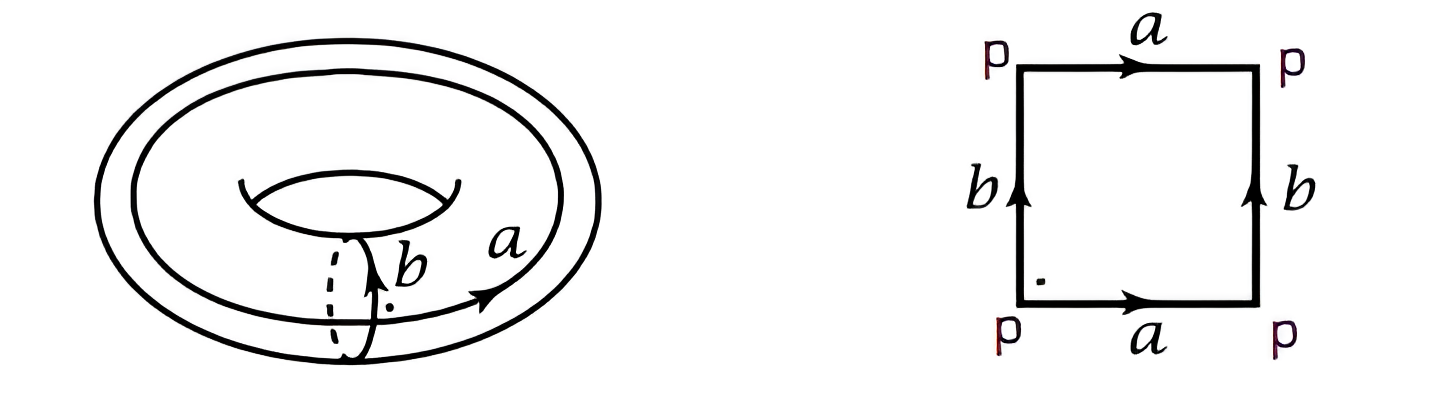
\includegraphics[height= 2.5cm]{torus.png}
    \caption{The torus $\mathbb{T}^2$ and its presentation as a cell complex (source: \cite{hatcher})}
    \label{fig:torus}
  \end{center}
\end{figure}
\\
In HoTT, this suggests the following definition by a HIT where we would manually fill the square:
\begin{itemize}
  \item $ p : \mathbb{T}^2$
  \item $a : p = p$
  \item $b : p = p $
  \item $\mathrm{fill} :  a \cdot b = b \cdot a$
\end{itemize}
And thanks to square types in cubical theory we can also give the following definition (in the cubical agda syntax, which should be readily understandable) : 
\begin{lstlisting}[mathescape=true]
    data Torus2 : Type where
    p : Torus2
    a : $ p \equiv p$
    b : $p \equiv p$
    fill : Square b b a a
\end{lstlisting}
Similarly, one can complete cubes in cubical type theory, but the structures involved quickly gain in complexity (but we shall look at such cubes later on).
\chapter{The Hypercubic manifold} 
In this part, we'll cover the work done during the internship. The formalized proofs and attempts of proofs can be found on the following GitHub repository \cite{repo}.
\section{Defining the hypercubic manifold}
The first part of the work was to give a formalized definition of the \textbf{hypercubic manifold}. As previously stated, this manifold can be obtained as the adjunction space of a 3-dimensional hypercub where opposite sides are identified with a quarter turn rotation. This is best illustrated in the following video \cite{VHvideo}. At the end of the day, it can be presented as the following object (illustration taken from \cite{hypercubic}):
\begin{figure}[h]
  \begin{center}
    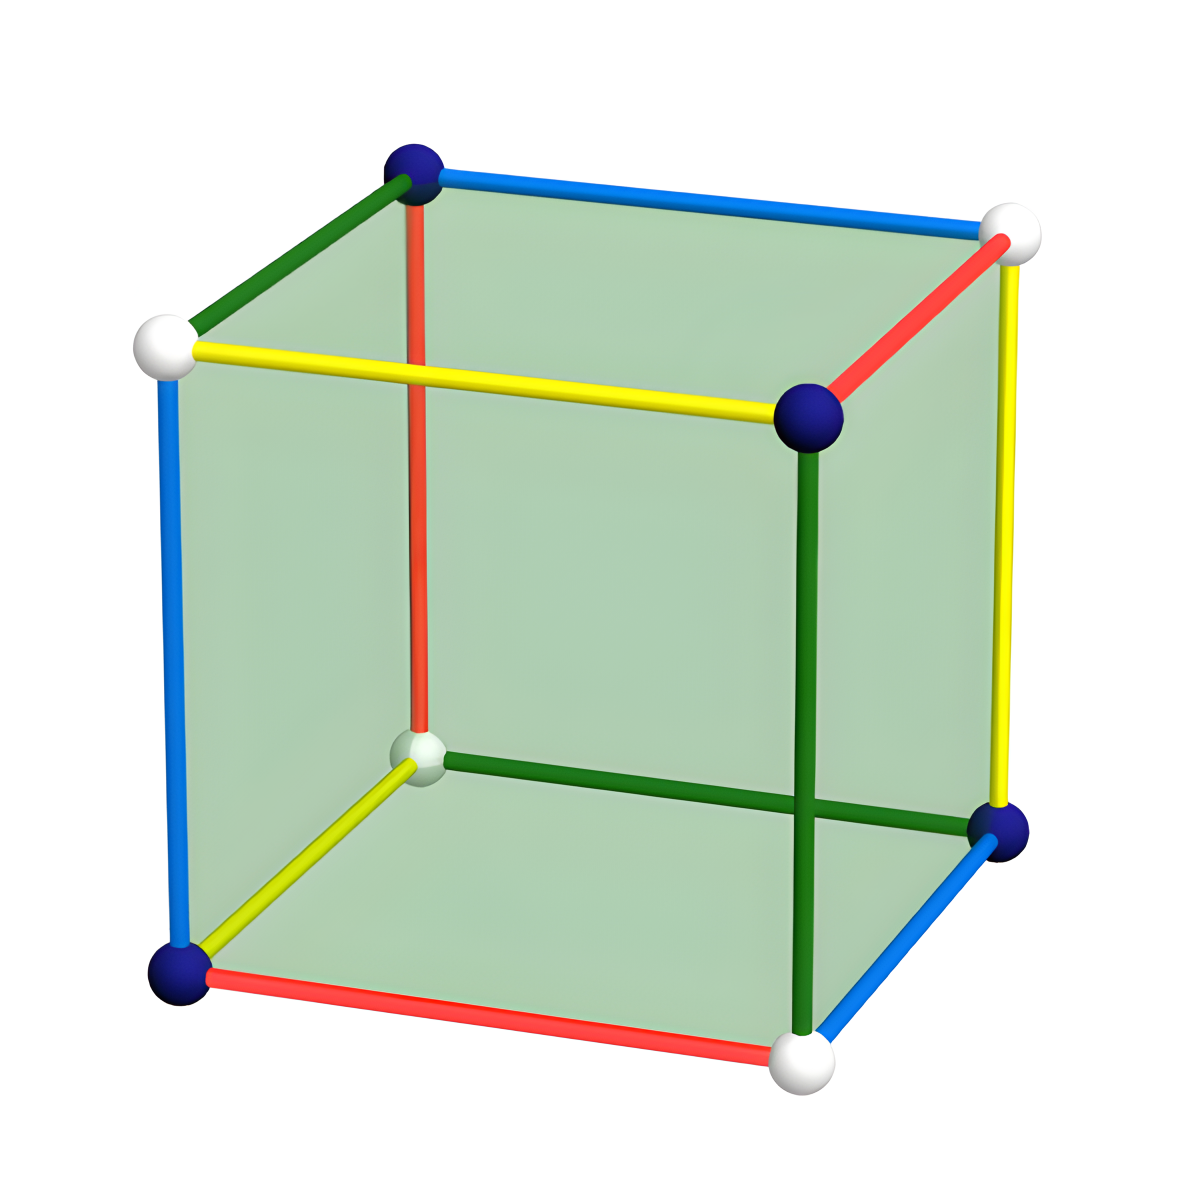
\includegraphics[height= 6.5cm]{cube-3-2.png}
    \caption{The hypercubic manifold}
    \label{fig:H1M}
  \end{center}
\end{figure}\\
Our goal is to define this object as a HIT, since we can already see what vertices,edges should be there. There are a few things that should be thought of however. First, this HIT would require filling a cube which can be a little tricky. Second, opposite faces are actually the same under a quarter turn rotation so this should also be sorted ouf within our HIT and this kind of structure didn't appear for the circle or the torus we previously saw. It should also be noted that filling squares is feasible in HoTT since it is tantamount to a commuting square of paths. However, filling cubes ought to be much more complicated since it deals with relations on squares. This is where cubical type theory comes in very handy for our purpose.\\
So, the first part of the work during this internship was to comprehend the specificites of cubical type theory (that were explained previously), getting familiar with filling squares and cubes to be able to tackle the more complex case of the hypercubic manifold. To do so, I defined a few different HITs involving increasingly difficult structures with squares, cubes or sides/edges being flipped to get as close as possible to our goal. All these HITs can be found in the GitHub repository \cite{repo} in "HiTs.agda". 
\newpage
\paragraph{The hypercubic manifold} For starters, let's name the vertice constructors $b^V$ and $w^V$ (for blue and white vertices) and the edge constructors $b^E$, $r^E$, $g^E$, $y^E$ (for blue,red,green,yellow edges) as figure 2.1 suggests. Now, a filled square : 
\begin{center}
  \begin{tikzcd}
    {} \arrow[r, "s"]                 & {}                 \\
    {} \arrow[u, "p"] \arrow[r, "r"'] & {} \arrow[u, "q"']
  \end{tikzcd}
\end{center}
is tantamount to having a relation $p \cdot s \equiv r \cdot q$. The latter can be rewritten $r^{-1} \cdot p \equiv q \cdot s^{-1}$ which gives us a filled square : 
\begin{center}
  \begin{tikzcd}
    {} \arrow[r, "p"]                      & {}                      \\
    {} \arrow[u, "r^{-1}"] \arrow[r, "q"'] & {} \arrow[u, "s^{-1}"']
    \end{tikzcd}
\end{center}
This allows us to define a quarter of a turn rotation operation on squares (where $\overline{p}$ denotes path inversion in cubical agda): 
$$\text{rot : Square $p$ $q$ $r$ $s$ $\rightarrow$ Square $\overline{r}$ $\overline{s}$ $q$ $p$}$$
This function can be synthetically defined as the following : $\boxed{\text{rot sq $i$ $j$ $:\equiv$ sq $(\sim j)$ $i$}}$. This map is naturally a quasi equivalence since $\mathrm{rot}^4\equiv \mathrm{Id}$, and its inverse is a quarter turn rotation in the other direction.\\
We now have every ingredient to define the hypercubic manifold. Let's first choose the orientation of our paths, $r^E$ and $b^E$ are chosen to be from $w^V$ to $b^V$ and $y^E$,$g^E$ are chosen to be in the other direction. Having chosen this direction, taking a look at the cubical documentation \cite{cubicalagda} (in Foundations/Prelude.agda) gives us the convention for filling cubes in agda, leading us to the following HIT:
\begin{figure}[h]
  \begin{center}
    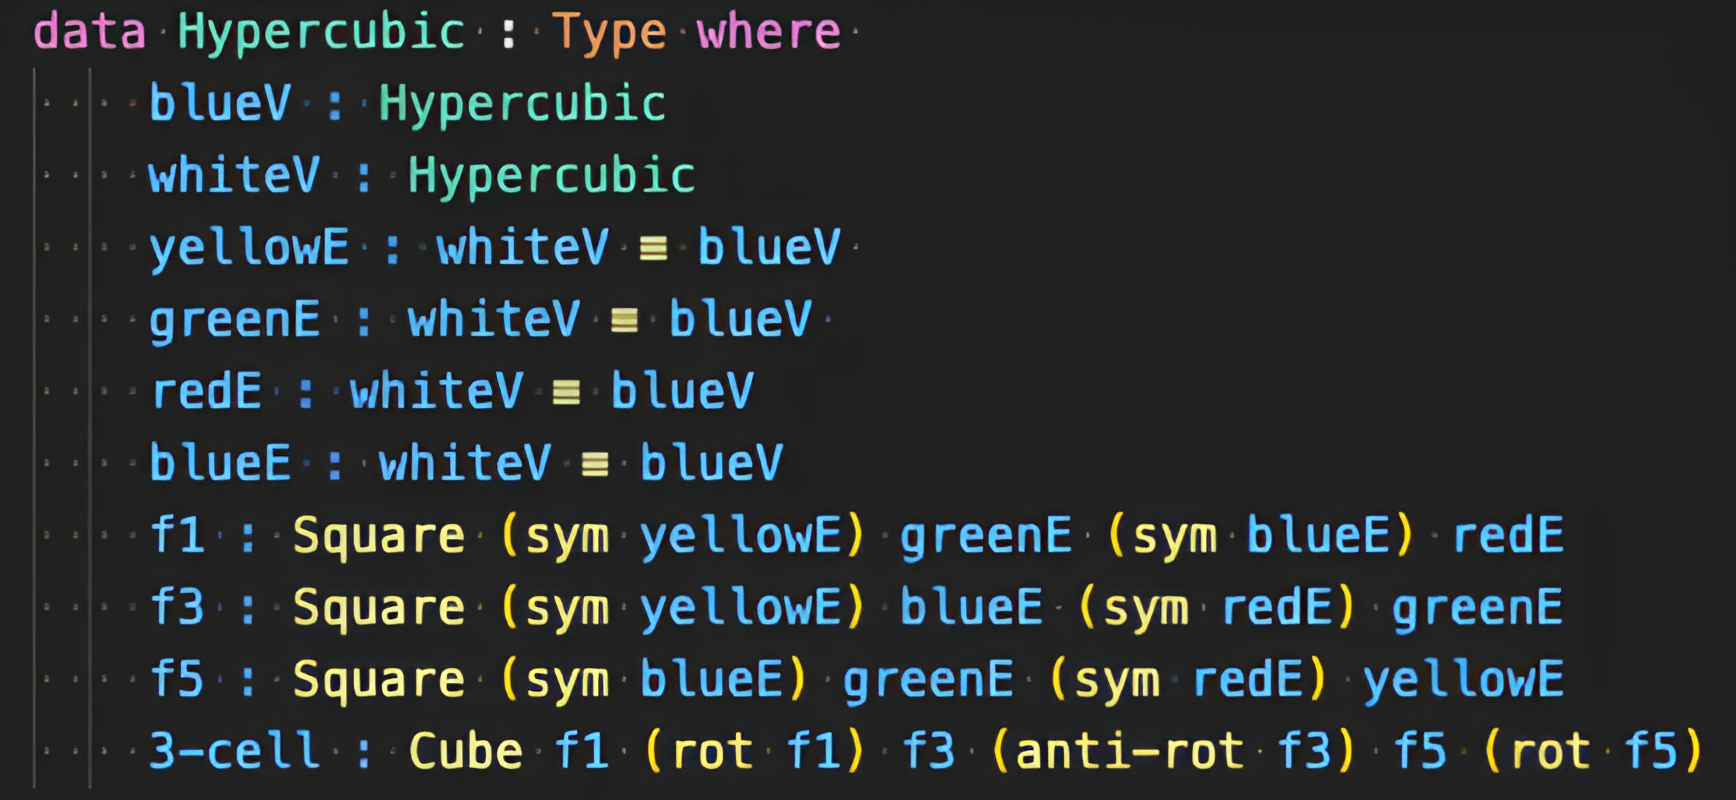
\includegraphics[height= 4.5cm]{images/Agda - VH.png}
    \caption{Synthetic description of the hypercubic manifold as a cubical HIT in cubical agda}
    \label{fig:H1Magda}
  \end{center}
\end{figure}\\
We shall now recover a known result about the fundamental group of the hypercubic manifold that we will denote by $\mathbb{HM}^1$ from now on. 
\begin{theorem}
  We have that $\pi_1(\mathbb{HM}^1)=\mathcal{Q}$ where $\mathcal{Q}$ is the quaternion group.
\end{theorem}
Before proving this claim we shall be taking a bit about \textbf{cell complexes} that we have first seen in \ref{fig:torus}. A cell complex is a topological space built inductively by successively attaching $0$-cells (points), $1$-cells (paths) and so on. In little dimensions, one can give them an abstract presentation as the one of the torus. The way these spaces are built should remind of higher inductive types, where one specifies some point constructors ($0$-paths), then path constructors ($1$-paths) and so on. In the section 6.6 of the HoTT book \cite{hott} one can find a bit more details about how a cell complex can be converted into a HIT. The idea is that attaching $n$-cells can be done by specifiying algebraic relations (such as $p \cdot q = q \cdot p$ for the torus) on lower dimensional constructors. It appears that the represenation of $\mathbb{HM}^1$ in \ref{fig:H1M} is also a cell-complex representation and that the cubical definition in \ref{fig:H1Magda} is precisely its conversion into a HIT.\\
Now, in classical homotopy theory the fact that $\pi_1(\mathbb{HM}^1)=\mathcal{Q}$ is well known and follows from a corollary of the \textbf{Seifert Van Kampen} theorem, stating that the fundamental group of a cell complex is given by the fundamental group of its $2$-skeleton (that is the complex where all cells of dimensions $>2$ are removed), more details can be found in \cite{hypercubic} and \cite{FundamentalCellComplex}. All we want to do here is check that the HIT we defined has the correct fundamental Then it can be shown that the fundamental group of a cell complex with one $0$-cell is given by the presentation $\langle S \hspace{2pt} \vert\hspace{2pt} R \rangle$ where you have one generator in $S$ for every $1$-cell and one relation for any $2$-cell.\\
Now, the relations that the $2$-cells should give are precisely the one used when you convert a cell complex into a HIT so we can indeed chack that the fundamental group of \ref{fig:H1Magda} is $\mathcal{Q}$ as it should be the case. 
\printbibliography

\end{document}
